\documentclass[12pt,a4paper,twoside]{article}

% Include packages that contain additional features, for example including special mathematical characters and images in your document
\usepackage{amssymb,amsmath,graphicx}
\usepackage[hidelinks]{hyperref}
\usepackage{verbatim}
%\usepackage{pdfpages}

\title{Exercises IV}
\author{Robin Greif (Exercise 3 Francisco Aros), Lia Hankla (Exercise 2 Victor Ksoll)}
\date{Due 2018/05/11}

\begin{document}
\maketitle

% Lab
\section{Exercise 1: Numerov Algorithm for the Schroedinger Equation}

\begin{figure}[h!]
  \centering
  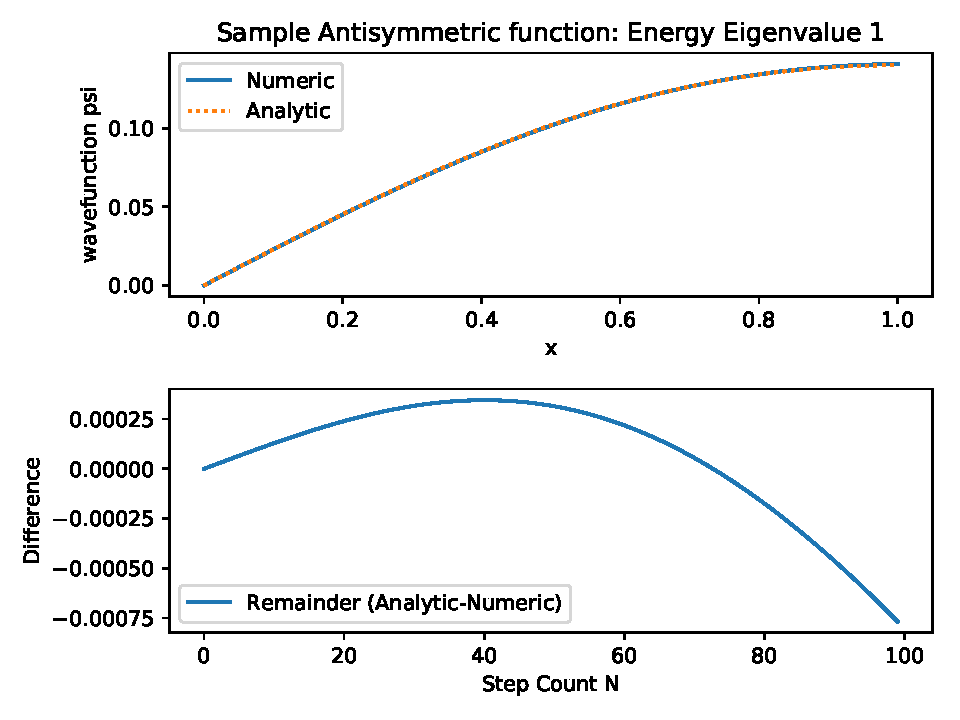
\includegraphics[width=.9\textwidth]{../exercise4_problem1_antisymEx.pdf}
  \caption{Antisymmetric solutions for harmonic oscillator using the Numerov Algorithm, compared to analytic solution} 
  \label{fig:1a}
\end{figure}

\begin{figure}[h!]
  \centering
  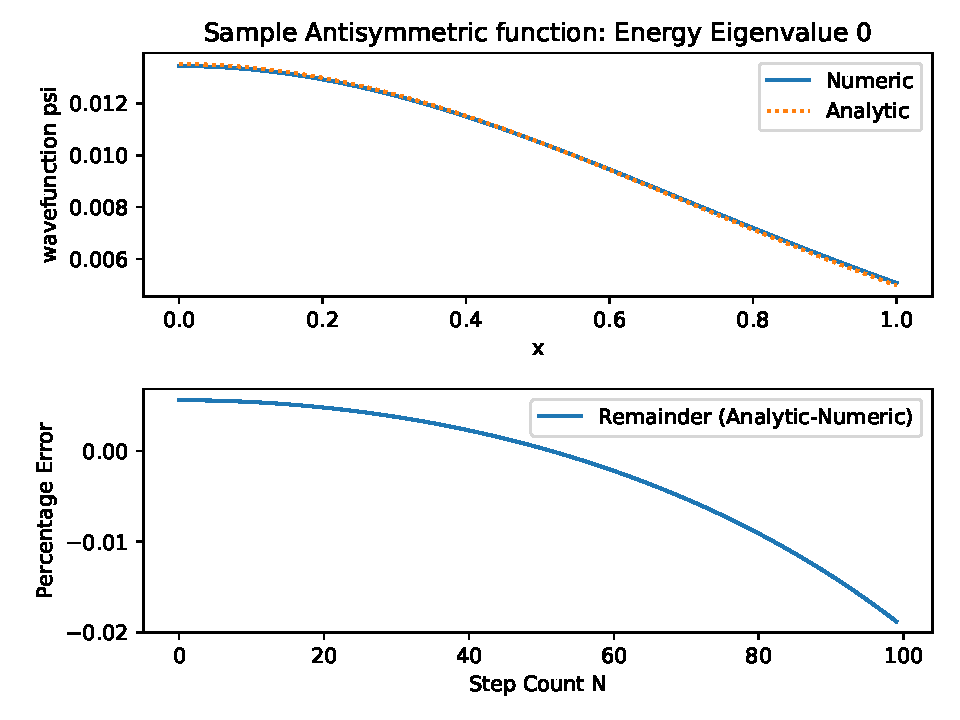
\includegraphics[width=.9\textwidth]{../exercise4_problem1_symEx.pdf}
  \caption{Symmetric solutions for harmonic oscillator using the Numerov Algorithm, compared to analytic solution} 
  \label{fig:1b}
\end{figure}


% Homework
\section*{Exercise 2: Neutrons in the grvitational field}

\begin{align*}
  0 &= \bigg(-\frac{\hbar^2}{2m} \frac{\partial^2}{\partialz^2} + mgz \bigg)
            \psi(z) - E \psi(z)  \\     
  0 &= \bigg(-\frac{\hbar^2}{2m} \frac{1}{R^2} \frac{\partial^2}{\partialz^2} + mgRx \bigg)
            \psi(x) - mgR\epsilon \psi(x)  \\       
  0 &= \psi''(x) + (\epsilon - x) \psi(x)  
\end{align*}

where we used
\begin{align*}
  R &= \bigg( \frac{\hbar^2}{2m^2g} \bigg) ^(1/3)  \\
  x &= z/R  \\
  \epsilon &= \frac{E}{mgR}  
\end{align*}


\subsection*{Part 1}




\subsection*{Part 2}


%
The code for the exercises is as follows:
\verbatiminput{../exercises04.py}




\end{document}

